\documentclass{beamer}



%\usepackage{txfonts}
\usepackage{kerkis}


\usepackage{beamerthemeblackboard}
\usepackage{environ}
%\usepackage{graphics}
%\usepackage{verbatim}

\usepackage[absolute,overlay]{textpos}
%\usepackage{tikz}
\setbeamertemplate{footline}{}





\newcommand{\mooculus}{\textsf{\textbf{MOOC}\textnormal{ULUS}}}



\newcommand{\MyBlock}[1]{
  \begin{textblock*}{\paperwidth}(0cm,8.5cm)
    \begin{tikzpicture}
      \node[rectangle, %rounded corners, 
        inner xsep=5pt,text width=\paperwidth,minimum height=.5in,align=right,anchor=west,
        text=yellow, text opacity=1,
        fill=black, fill opacity=.8](box){
        \hfill\raisebox{10pt}{\scalebox{2}{ #1 \quad}}
      };
    \end{tikzpicture}

  \end{textblock*}
}



%% \newcommand{\MyBlock}[1]{
%%   \begin{textblock*}{11cm}(1cm,8.5cm)
%%     \hfill\scalebox{2}{\color{red!70!black} #1}
%%   \end{textblock*}
%% }






\usebackgroundtemplate%
{%
    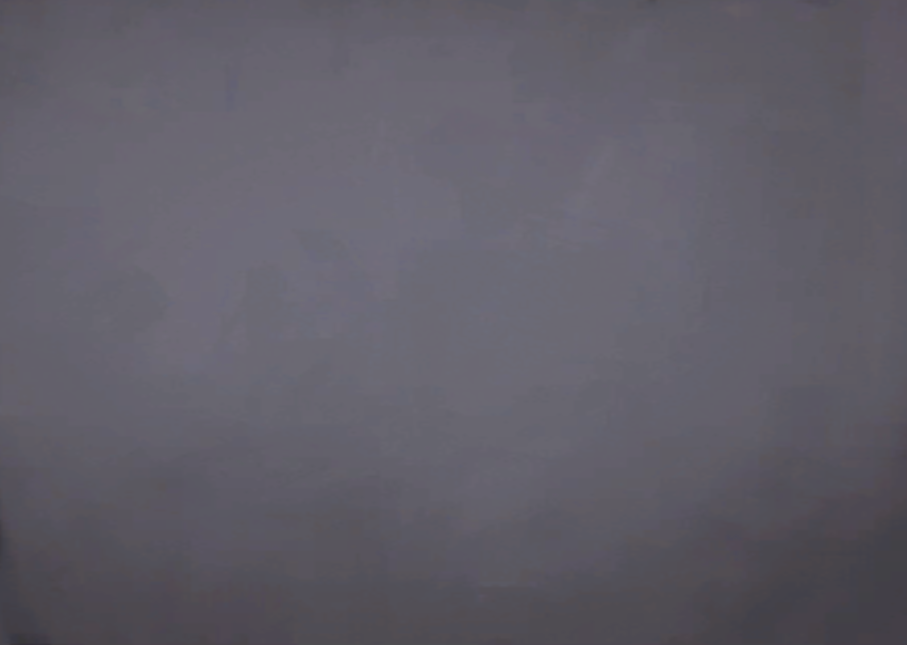
\includegraphics[width=\paperwidth,height=\paperheight]{blackboard.png}%
}
\begin{document}



\title{\scalebox{2}{\mooculus}}
\author{Massive Open Online Calculus}
\date{}
\begin{frame}
\titlepage
\end{frame}







{
\usebackgroundtemplate{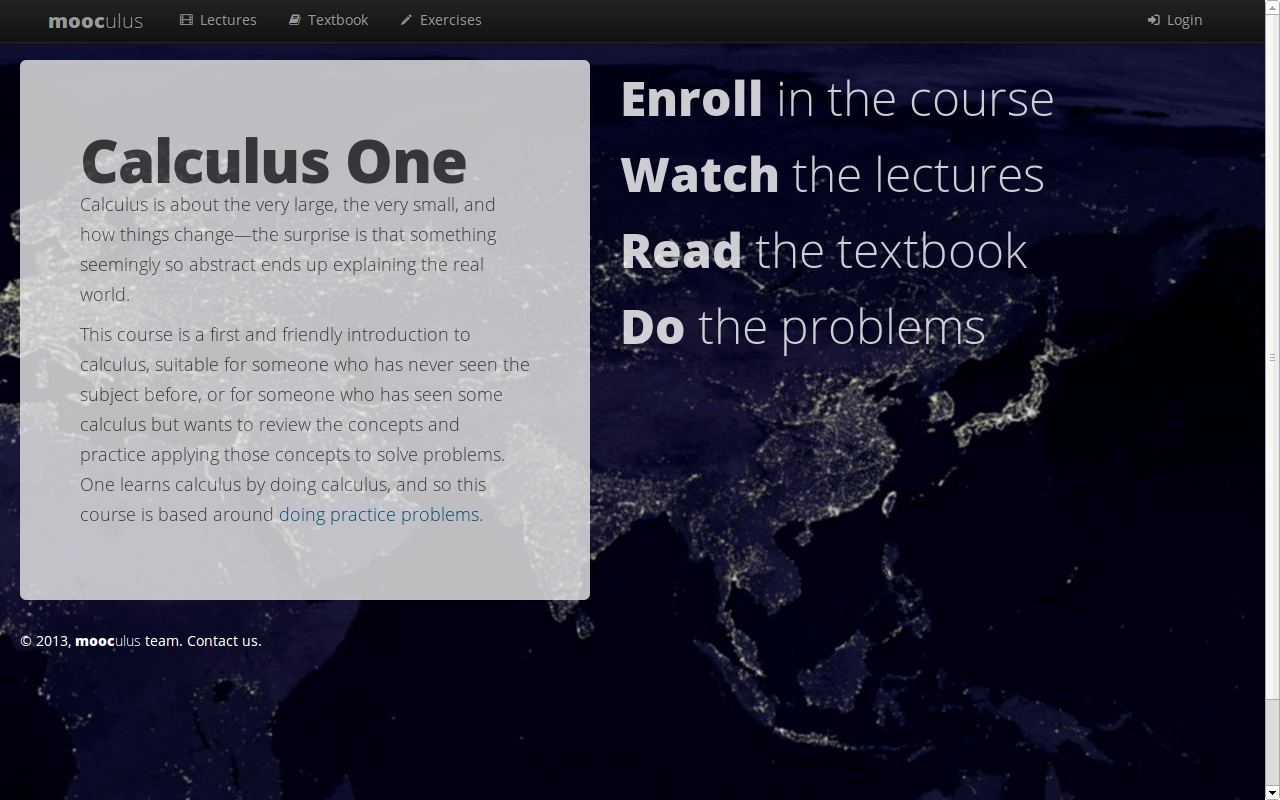
\includegraphics[height=\paperheight]{mooculusHome.png}}
\begin{frame}

\MyBlock{What is \mooculus?}
\end{frame}
}





{
\usebackgroundtemplate{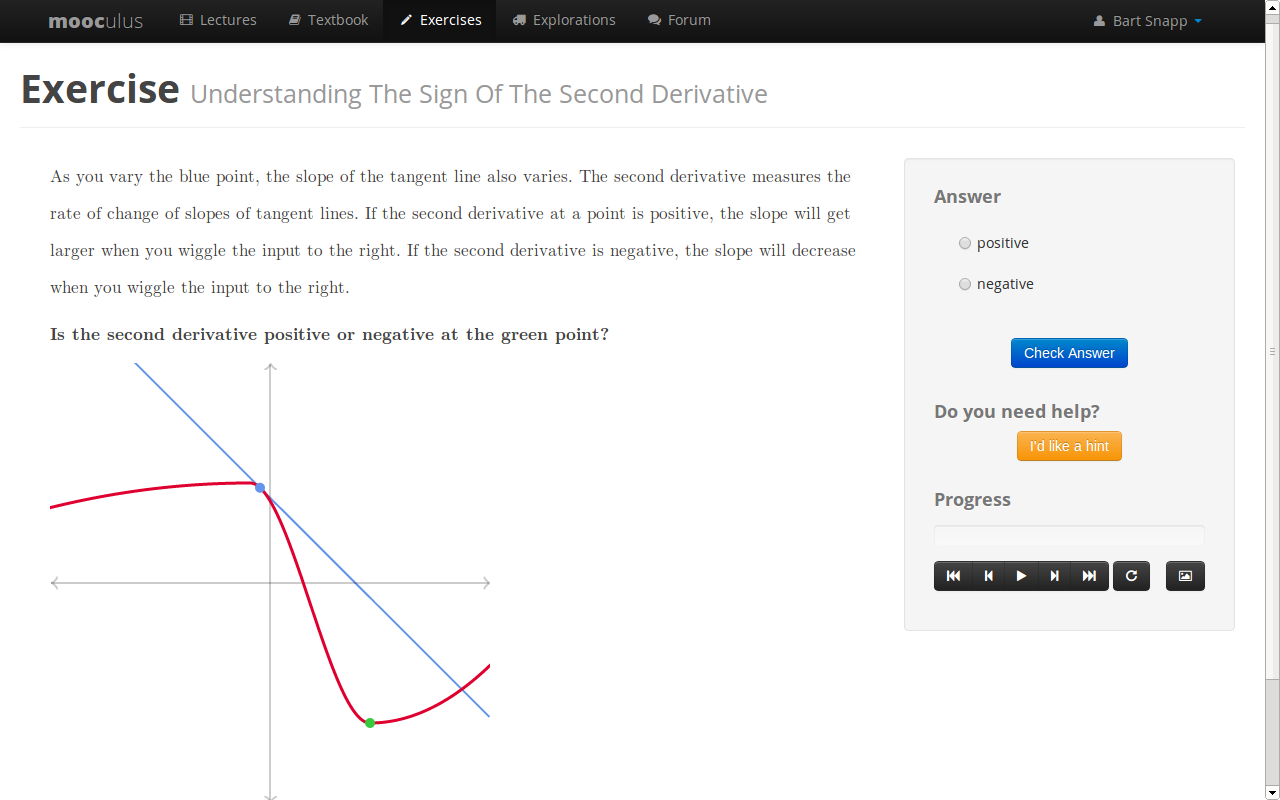
\includegraphics[height=\paperheight]{exercise.png}}
\begin{frame}

\MyBlock{What is \mooculus?}
\end{frame}
}


{
\usebackgroundtemplate{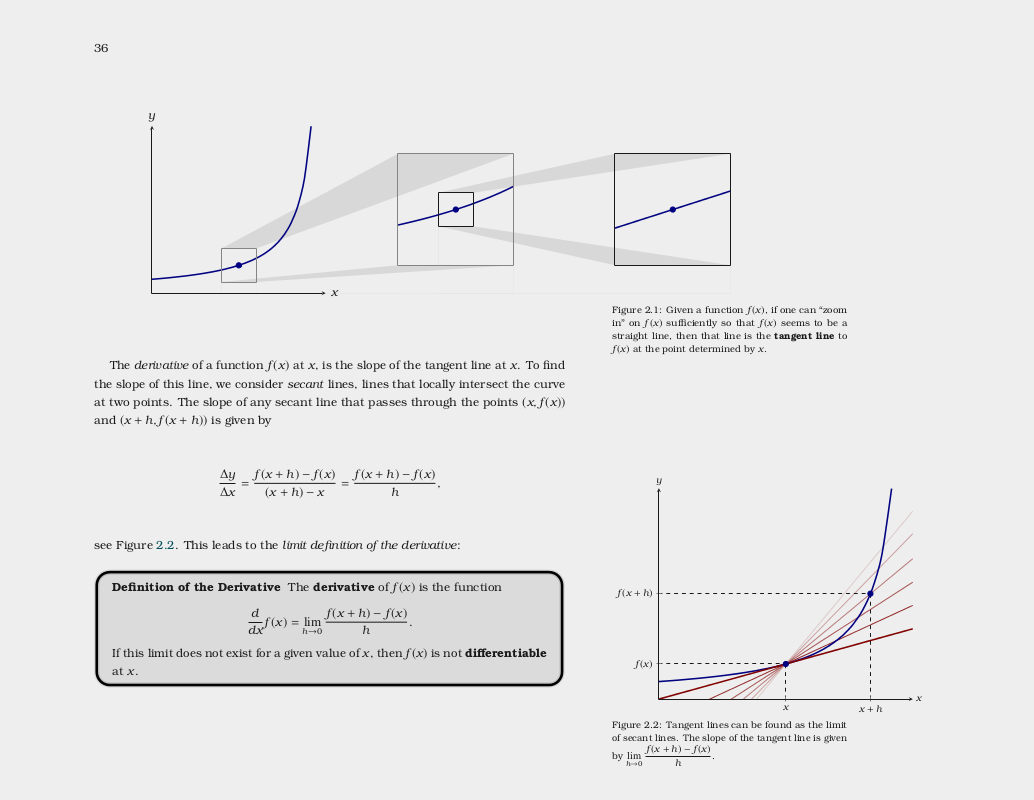
\includegraphics[width=\paperwidth]{textbook.png}} %% NEED TO ZOOM!
\begin{frame}

\MyBlock{What is \mooculus?}
\end{frame}
}

{
\usebackgroundtemplate{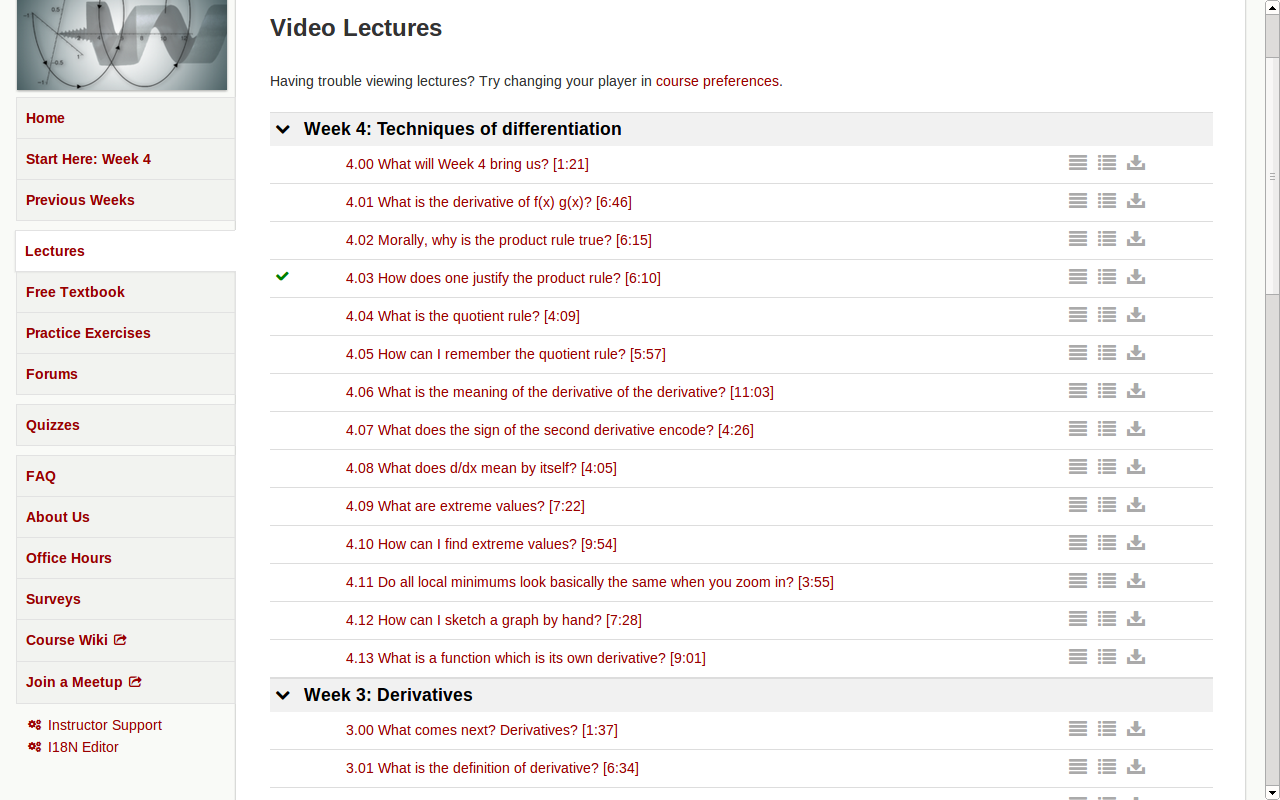
\includegraphics[height=\paperheight]{lectures.png}}
\begin{frame}

\MyBlock{What is \mooculus?}
\end{frame}
}


{
\usebackgroundtemplate{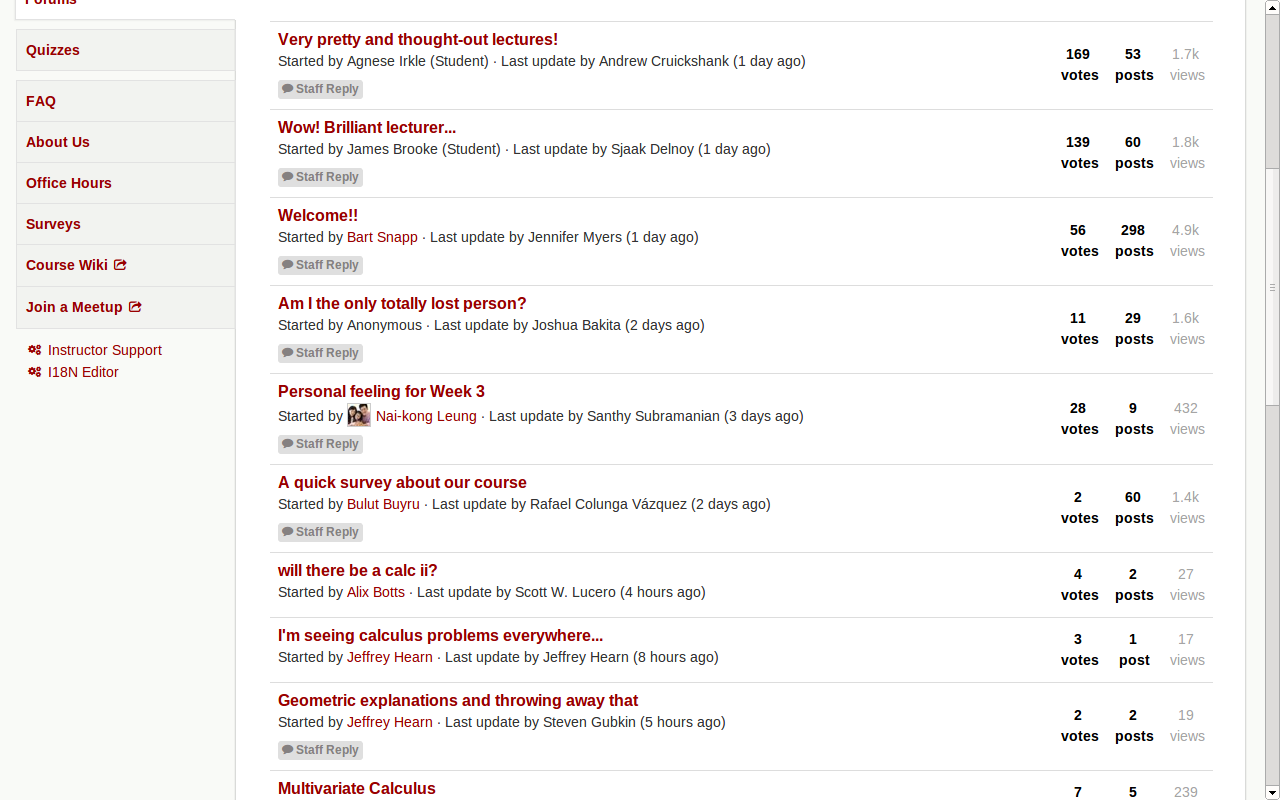
\includegraphics[height=\paperheight]{forum.png}}
\begin{frame}

\MyBlock{What is \mooculus?}
\end{frame}
}



{
\usebackgroundtemplate{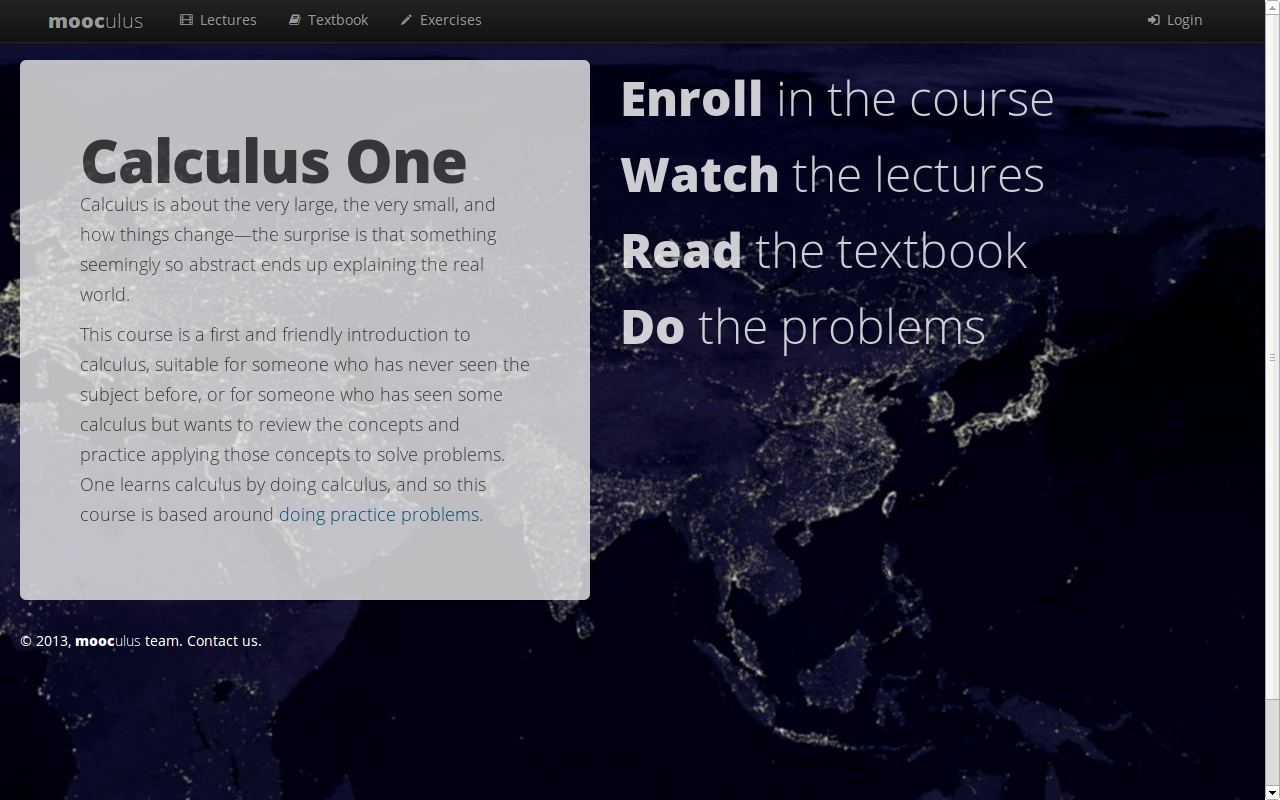
\includegraphics[height=\paperheight]{mooculusHome.png}}
\begin{frame}

\MyBlock{How do students use \mooculus?}
\end{frame}
}


{
\usebackgroundtemplate{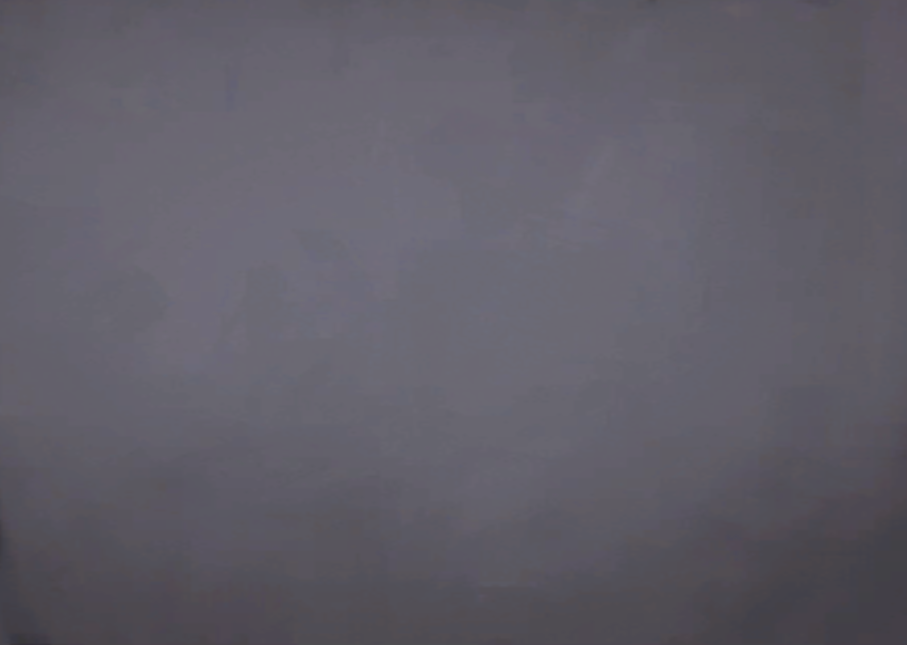
\includegraphics[height=\paperheight]{blackboard.png}}
\begin{frame}
\begin{center}
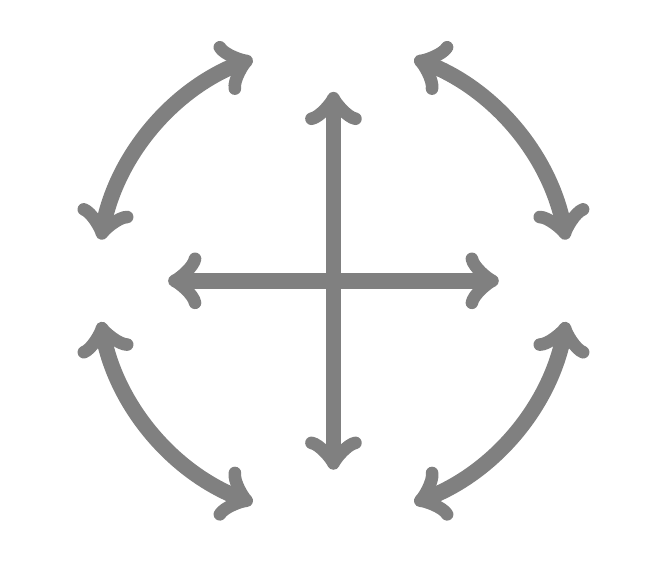
\begin{tikzpicture}[scale=3]
%\draw[help lines] (0,0) grid (5,4);
\draw [gray,<->,line width=2mm] (.342,.940) arc [radius=1, start angle=70, end angle =10];
\draw [gray,<->,line width=2mm] (.985,-.174) arc [radius=1, start angle=-10, end angle =-70];
\draw [gray,<->,line width=2mm] (-.342,-.940) arc [radius=1, start angle=250, end angle =190];
\draw [gray,<->,line width=2mm] (-.9850,.174) arc [radius=1, start angle=170, end angle =110];

\draw [gray,<->,line width=2mm] (-.7,0)--(.7,0);
\draw [gray,<->,line width=2mm] (0,.8)--(0,-.8);


\node at (0,1) [white] {\textbf{Lectures}};
\node at (1,0) [white] {\textbf{Textbook}};
\node at (-1,0) [white] {\textbf{Exercises}};
\node at (0,-1) [white] {\textbf{Forum}};
\end{tikzpicture}
\end{center}
\MyBlock{How do students use \mooculus?}
\end{frame}
}

{
\usebackgroundtemplate{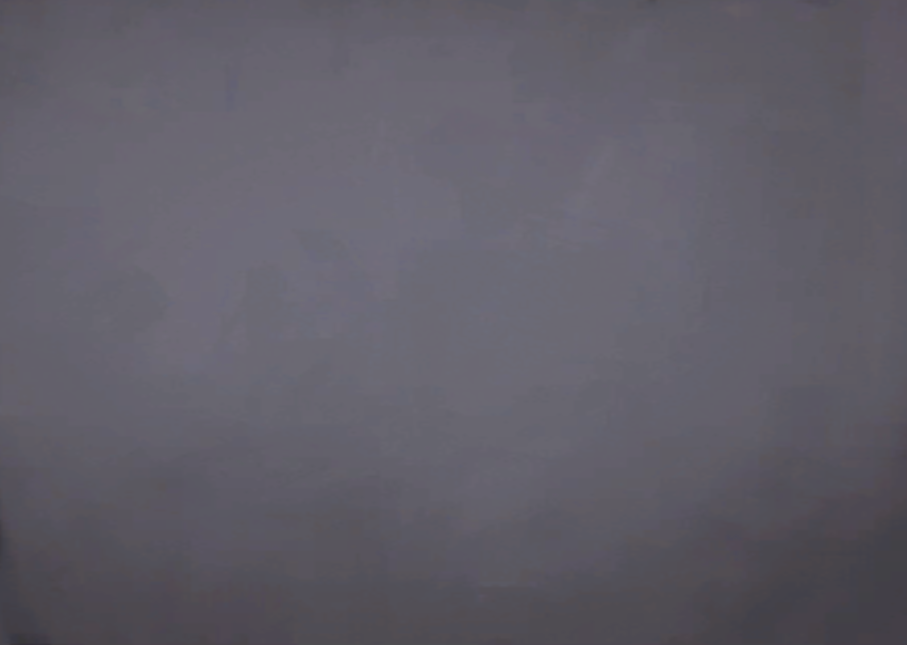
\includegraphics[height=\paperheight]{blackboard.png}}
\begin{frame}

\scalebox{1.5}{\textbf{As a way to flip a classroom.}}

\vspace{10pt}

\scalebox{1.5}{\textbf{As a supplement to high school courses.}}

\vspace{10pt}

\scalebox{1.5}{\textbf{As a supplement to courses at other colleges.}}

\vspace{10pt}

\scalebox{1.5}{\textbf{As an online course with in class exams.}}

\vspace{10pt}

\scalebox{1.5}{\textbf{As a total online course.}}

\vspace{10pt}

\MyBlock{Where will \mooculus~take us?}
\end{frame}
}


{
\usebackgroundtemplate{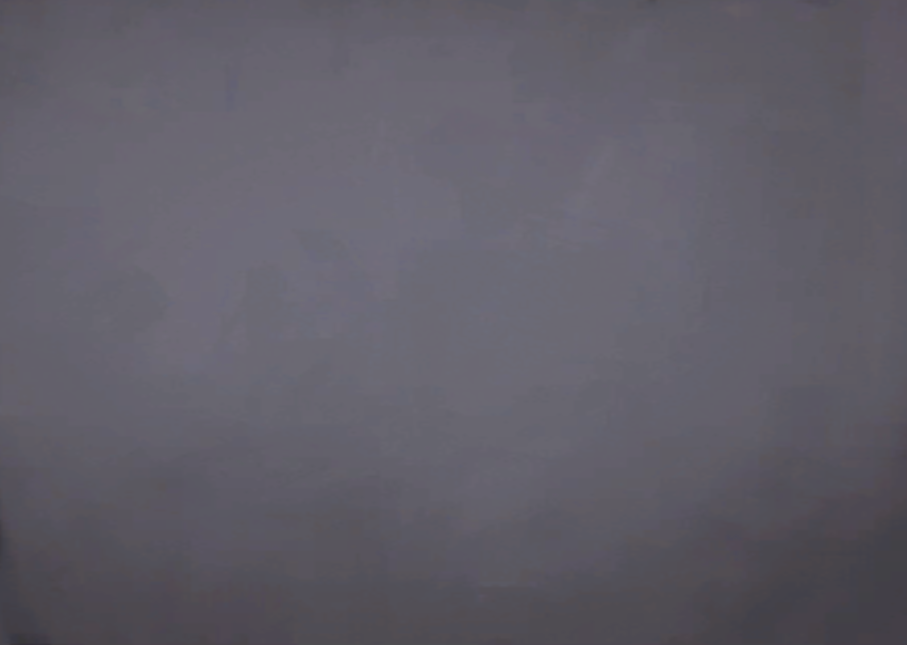
\includegraphics[height=\paperheight]{blackboard.png}}
\begin{frame}

\scalebox{1.5}{\textbf{Analytics for Research}}

\vspace{10pt}

\scalebox{1.5}{\textbf{Mastery of Skills}}

\MyBlock{Where will \mooculus~take us?}
\end{frame}
}


\end{document}
